%%%%%%%%%%%%%%%%%%%%%%%%%%%%%%%%%%%%%%%%%%%%%%%%%%%%%%%%%%%%%%%%%%%%%%
% How to use writeLaTeX: 
%
% You edit the source code here on the left, and the preview on the
% right shows you the result within a few seconds.
%
% Bookmark this page and share the URL with your co-authors. They can
% edit at the same time!
%
% You can upload figures, bibliographies, custom classes and
% styles using the files menu.
%
% If you're new to LaTeX, the wikibook is a great place to start:
% http://en.wikibooks.org/wiki/LaTeX
%
%%%%%%%%%%%%%%%%%%%%%%%%%%%%%%%%%%%%%%%%%%%%%%%%%%%%%%%%%%%%%%%%%%%%%%
\documentclass{tufte-handout}

%\geometry{showframe}% for debugging purposes -- displays the margins

\usepackage{amsmath}

% Set up the images/graphics package
\usepackage{graphicx}
\setkeys{Gin}{width=\linewidth,totalheight=\textheight,keepaspectratio}
\graphicspath{{graphics/}}




%Portuguese-specific commands
%--------------------------------------
\usepackage[portuguese]{babel}
%--------------------------------------
 
%Hyphenation rules
%--------------------------------------
\usepackage{hyphenat}
\hyphenation{mate-mática recu-perar}
%--------------------------------------


% fix pro tufte no xetex (q preciso para fontes customizadas)
% https://tex.stackexchange.com/a/202189
\usepackage{ifxetex}
\ifxetex
  \newcommand{\textls}[2][5]{%
    \begingroup\addfontfeatures{LetterSpace=#1}#2\endgroup
  }
  \renewcommand{\allcapsspacing}[1]{\textls[15]{#1}}
  \renewcommand{\smallcapsspacing}[1]{\textls[10]{#1}}
  \renewcommand{\allcaps}[1]{\textls[15]{\MakeTextUppercase{#1}}}
  \renewcommand{\smallcaps}[1]{\smallcapsspacing{\scshape\MakeTextLowercase{#1}}}
  \renewcommand{\textsc}[1]{\smallcapsspacing{\textsmallcaps{#1}}}
  \usepackage{fontspec}
\fi


\usepackage{fontspec}
\setmainfont[
    Path=./Literata/,
    BoldFont=Literata-Bold,
    ItalicFont=Literata-Italic,
    BoldItalicFont=Literata-BoldItalic,
]{Literata-Regular}

\title{Letras que ecoem a fala: tipografia modulada por prosódia}
%\title{A voz na letra: tipografia modulada pela fala}

\author{Caluã de Lacerda Pataca, Paula Dornhofer Paro Costa}
\date{24 de novembro de 2019}  % if the \date{} command is left out, the current date will be used

% The following package makes prettier tables.  We're all about the bling!
\usepackage{booktabs}

% The units package provides nice, non-stacked fractions and better spacing
% for units.
\usepackage{units}

% The fancyvrb package lets us customize the formatting of verbatim
% environments.  We use a slightly smaller font.
\usepackage{fancyvrb}
\fvset{fontsize=\normalsize}

% Small sections of multiple columns
\usepackage{multicol}

% Provides paragraphs of dummy text
\usepackage{lipsum}

% These commands are used to pretty-print LaTeX commands
\newcommand{\doccmd}[1]{\texttt{\textbackslash#1}}% command name -- adds backslash automatically
\newcommand{\docopt}[1]{\ensuremath{\langle}\textrm{\textit{#1}}\ensuremath{\rangle}}% optional command argument
\newcommand{\docarg}[1]{\textrm{\textit{#1}}}% (required) command argument
\newenvironment{docspec}{\begin{quote}\noindent}{\end{quote}}% command specification environment
\newcommand{\docenv}[1]{\textsf{#1}}% environment name
\newcommand{\docpkg}[1]{\texttt{#1}}% package name
\newcommand{\doccls}[1]{\texttt{#1}}% document class name
\newcommand{\docclsopt}[1]{\texttt{#1}}% document class option name

\begin{document}

\maketitle% this prints the handout title, author, and date

\begin{abstract}
\noindent Hello World.
\end{abstract}

%\printclassoptions

\section{Objetivos e justificativas do projeto de pesquisa}\label{sec:objetivos}
%\subsection{Headings}\label{sec:headings}


\section{Revisão bibliográfica resumida}\label{sec:revisao_bibliografica}

Prosódia enquanto dimensão linguística, paralinguística, extralinguística.

Prosódia diz respeito não só ao que se fala e se ouve, mas também ao que se lê.

Estudo da Ann Bessemans.

Prosódia enquanto desambiguação, interrogação, exclamação etc. A tipografia entra nisso como? (História do espaço, pontuações, talvez algo sobre tone of voice)

Prosódia como representação do estado emocional do falante. Estudo do Plínio.

Discussão sobre emoção interpretada vs representação de atributos acústicos.

Discussão sobre legendas.

\section{Metodologia utilizada}\label{sec:metodologia}

\subsection{Extração e representação de prosódia}\label{sec:met_extract_represent}

\subsection{Experimento \#1: Card sorting e entrevistas com designers}\label{sec:met_exp_2}

\subsection{Experimento \#2: Associação entre emoções, \textit{features} prosódicas e eixos tipográficos}\label{sec:met_exp_2}

\subsection{Experimento \#3: }\label{sec:met_exp_2}

\section{Plano de trabalho e cronograma}\label{sec:plano_de_trabalho}

\section{Resultados e conclusões parciais}\label{sec:resultados}

\subsection{O primeiro experimento}

Os resultados do primeiro experimento talvez valham mais pelo que as entrevistas revelaram do que propriamente pelas \textit{edit-distances} medidas nas organizações dos cartões. Estas deveriam medir se os participantes conseguiram intuir na tipografia aspectos do estado emocional da voz da atriz que leu  as frases impressas nos cartões, mas o efeito capturado foi muito pequeno: a \textit{edit-distance} média no experimento é, na média, apenas 2\% menor que a que se poderia esperar caso os participantes simplesmente sorteassem as posições de cada cartão (cf. Figura~\ref{edit_dist_1}).

\begin{marginfigure}
  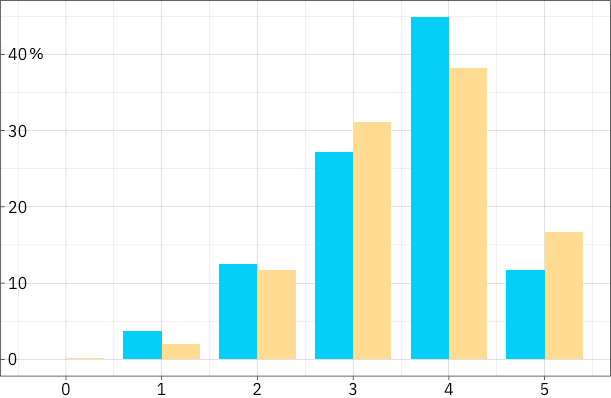
\includegraphics{imgs/edit_distance_reais.png}
  \caption{\textit{Edit-distances} das organizações coletadas (em azul) \textit{vs} uma organização ``aleatória'' (em amarelo).}
  \label{edit_dist_1}
\end{marginfigure}

Aqui, não pudemos intuir se nos dados estávamos vendo que nossa tipografia modulada pela fala era ineficaz ou se estávamos sofrendo com o mau desenho do experimento. Talvez, apostamos, seja mais o segundo caso: o modo como configuramos o \textit{card sort} pode ter conduzido a altas taxas de erro. Como \textit{todos} os cartões deveriam necessariamente ser atribuídos a uma emoção, estão embaralhados em nossos resultados coletados tanto cartões em que o participante tinha algum grau de certeza sobre a emoção quanto aqueles em que houve um ``chute.''\sidenote[][-1\baselineskip]{E, para piorar, no \textit{card sort} um cartão errado implicará necessariamente em um segundo cartão também errado.} Temos motivos para crer que esses chutes foram comuns, pois, tanto nas entrevistas quanto espontaneamente durante a atividade, muitos participantes nos relataram que a atividade era muito difícil.

A essa dificuldade da atividade em si soma-se o fato de que misturamos no experimento, e sem nenhuma forma de controle que isolassem seus efeitos, variações de três \textit{features} prosódicas com três eixos tipográficos associados a seis emoções. Dado esse cenário, não é de se espantar que com os dados coletados nos foi muito difícil responder quão bem (ou mal) nosso modelo prosódico-tipográfico representava a voz da atriz em cada uma das emoções presentes. 


\begin{marginfigure}
  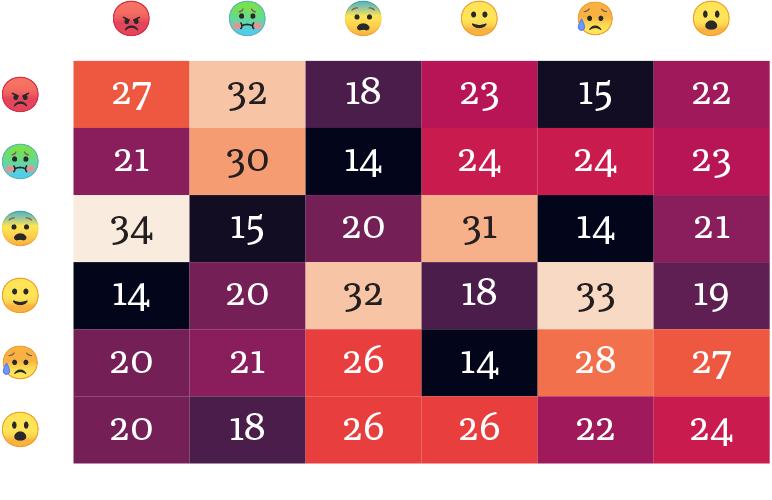
\includegraphics{imgs/confusion-emoji2.png}
  \caption{Matriz de confusão do experimento de \textit{card sort}. Emoção da atriz nas linhas, classificação dos participantes nas colunas.}
  \label{matriz_confusao}
\end{marginfigure}

Na tentativa de encontrar explicações alternativas para o baixo ganho no \textit{edit-distance}, nos perguntarmos se certos aspectos do modelo prosódico-tipográfico não estariam fazendo os participantes trocarem uma emoção por outra. Esta hipótese nos ocorreu na análise da matriz de confusão da Figura~\ref{matriz_confusao}, que parece indicar uma possível troca feita pelos participantes especificamente entre os cartões representando medo e alegria (terceira e quarta linhas e colunas). Teria o modelo invertido o sentido de alguma das features ou eixos tipográficos em relação ao que seria intuitivo? Para testar a hipótese, calculamos novamente a \textit{edit-distance}, desta vez considerando que os cartões com medo seriam de alegria e vice-versa. Como mostra a Figura~\ref{edit_dist_2}, a performance melhora (8\% de ganho em relação à distribuição aleatória). Mas o efeito continua pequeno.

\begin{marginfigure}[0.5\baselineskip]
  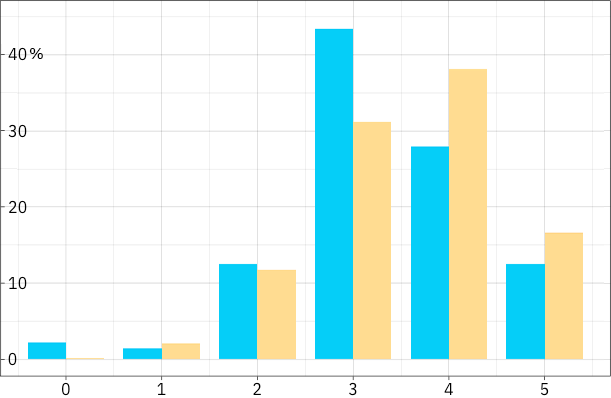
\includegraphics{imgs/edit_distance_troca.png}
  \caption{\textit{Edit-distances} das organizações coletadas, mas com troca alegria--medo (em azul) \textit{vs} uma organização ``aleatória'' (em amarelo).}
  \label{edit_dist_2}
\end{marginfigure}

O que nos disseram as entrevistas? Além do muito frequente comentário de que a avaliação era muito difícil, emergiram alguns padrões em como os participantes interpretaram as modulações tipográficas. De longe o atributo mais citado, aumento no \textit{peso} foi quase unanimemente associado a maior volume na voz, ainda que foram poucos os que perceberam que pesos leves estavam relacionados a volumes baixos na voz.

Em relação aos outros dois eixos houve grande difusão de comentários. Sobre a \textit{inclinação}, houve quem a interpretasse como velocidade, fraqueza, tristeza, ou mesmo alguns que notaram as modulações nesse eixo mas que não souberam decodificá-las. \textit{Largura} foi citada por apenas um participante, que intuiu corretamente que seu aumento e baixa estavam relacionados a oscilações de duração na pronúncia das sílabas.

Comentando sobre estratégias usadas para classificar cada cartão, emergiram dois principais grupos: no primeiro, mais frequente, o participante olhava para o cartão e buscava ``soá-lo'' mentalmente\sidenote{Ou, mais raramente, em voz baixa, como notamos em alguns casos.}, tentando interpretar em sons as modulações visuais nas letras. O segundo grupo ia no sentido oposto: tentava fazer soar a frase como que sob o efeito de cada uma das seis emoções para só então buscar nos cartões aquele cuja tipografia se aproximasse do som.

Como muitos participantes sequer perceberam as modulações de \textit{largura} e que houve grande divergência em como foram interpretadas as modulações de \textit{inclinação}, podemos supor que ambas as estratégias relatadas sofrem de um mesmo problema: se apenas os momentos mais gritados foram bem capturados, grande parte da expressividade na voz da atriz se perdeu e, não só isso, essa perda compromete de maneira desigual cada uma das emoções\sidenote[][-1\baselineskip]{Cf. o artigo de ..., que mostra como diferentes emoções são expressas em diferentes dimensões prosódicas.}.

\subsection{O segundo experimento}

\renewcommand{\refname}{Bibliografia}
\makeatletter
\renewcommand{\bibsection}{%
   \section{\refname%
            \@mkboth{\MakeUppercase{\refname}}{\MakeUppercase{\refname}}%
   }
}
\makeatother


\bibliography{sample-handout}
\bibliographystyle{plainnat}



\end{document}